\documentclass{beamer}
\usepackage{graphicx}
% Theme
\usetheme{default}
\usecolortheme{lily}
% Title page
\title{Super Resolution Image Processing using GenAI}
\author{Mrunmayee \and Ruchi  \and Udita}
\institute{WE Cohort V}
\date{\today}

\begin{document}
\maketitle

%\begin{frame}
%  \titlepage
%\end{frame}

% Problem statement
%\begin{frame}{Research Topic}
  %\begin{itemize}
   % \item Creating a fashion recommendation website.
   % \item In the age of online shopping, users often face decision fatigue and the overwhelming task of sifting through countless options on various e-commerce platforms. 
  %\end{itemize}
%\end{frame}

% Tech Stack
\begin{frame}{About}
  \begin{itemize}
    \item Image Super-Resolution enhances image resolution by 4x+. Its various applications include improving image quality, enhancing visual detail, and increasing the accuracy of computer vision algorithms.
  \end{itemize}
\end{frame}

% Objectives
\begin{frame}{Data Processing Inequality}
  \begin{itemize}
    \item According to Information Theory , whatever way we process data we cannot add information that is not already present.
    \item This implies that missing data cannot be recovered from further data processsing.
  \end{itemize}
\end{frame}

% Objectives
\begin{frame}{Use of AI}
  \begin{itemize}
    \item This is where Neural Networks enter the picture. These are trained on a large set of images and learn to hallucinate details based on this prior information.
    \item The details thus added do not violate the data processing inequality.
    
  \end{itemize}
\end{frame}

% Objectives
\begin{frame}{What are Neural Networks }
  \begin{itemize}
    \item An artificial neural network is made of artificial neurons that work together to solve a problem. Artificial neurons are software modules, called nodes, and artificial neural networks are software algorithms that use computing systems to solve mathematical calculations at core. 
    \item{}
    
 \end{itemize} 
\begin{tabular}{lll}
\textbf{Layer} & \textbf{Description} & \textbf{Function} \\ \hline
Input Layer & Receives external information  & Processes and transmits data \\
Hidden Layer(s) & (Optional) Processes information from previous layers  & Analyzes and transforms data \\
Output Layer & Provides final result  & Generates classification or prediction
\end{tabular}

\end{frame}
% Objectives
\begin{frame}{Convulational Neural Networks}
  \begin{itemize}
    \item The hidden layers in convolutional neural networks perform specific mathematical functions, like summarizing or filtering, called convolutions. 
    \item They are very useful for image classification because they can extract relevant features from images that are useful for image recognition and classification. 
    \item This new form is easier to process without losing features that are critical for making a good prediction. Each hidden layer extracts and processes different image features, like edges, color, and depth.
    
    
  \end{itemize}
\end{frame}

\begin{frame}{SRCNN}
  \begin{itemize}
    \item Super-Resolution Convolutional Neural Network : a pioneering deep learning model designed for image super-resolution 
    \item Enhances the resolution of images by learning end-to-end mappings from low-resolution to high-resolution images using convolutional neural networks 
    \item comprises three key steps: patch extraction and representation, non-linear mapping, and reconstruction
    
  \end{itemize}
\end{frame}
% Objectives
\begin{frame}{Loss Functions}
  \begin{itemize}
    \item It's a mathematical function that quantifies the difference between a model's predictions and the actual target values.
    \item Lower scores indicate the model's doing well. The loss function uses this difference to tell the model how to adjust itself. By minimizing the loss, the model learns to make more accurate predictions.
    
    
    
  \end{itemize}
\end{frame}
% Objectives
\begin{frame}{Choosing the right loss function}
  \begin{itemize}
    \item MSE: Focuses on pixel-level differences between the generated image and the ground truth (actual high-resolution image). It calculates the average squared difference between corresponding pixels.
    \item SSIM: Goes beyond pixel values and considers structural similarity. It analyzes the image in terms of luminance (brightness), contrast, and structure, providing a more human-centric evaluation of image quality.
    \item A new, differentiable error function specifically designed for image restoration tasks which aims to combine the benefits of both MSE and perceptual losses lead to significantly better image restoration results.
    
    
    
  \end{itemize}
\end{frame}

\begin{frame}{GANs}
  \begin{itemize}
    \item Its a powerful architecture which works on the principle of  constant competition between two neural networks 
    \item Generator: This network acts like an artist, constantly trying to create new, realistic images that could be mistaken for real examples.
    \item Discriminator: This network acts like a critic, meticulously analyzing the data generated by the generator and trying to distinguish it from real data.
    
  \end{itemize}
\end{frame}

\begin{frame}
  \LARGE{Demo}
\end{frame}

\begin{frame}{Interseting Usecase}
  \begin{itemize}
    \item Pixel 3 uses Super resolution for better Zoom effect 
    \item Statement from an article,"The Super Res Zoom technology in Pixel 3 is different and better than any previous digital zoom technique based on upscaling a crop of a single image, because we merge many frames directly onto a higher resolution picture"
    \item thus zoom option becomes better than cropping the image afterwards
  \end{itemize}
\end{frame}

\begin{frame}{Algorithm used}
  \begin{figure}
      \centering
      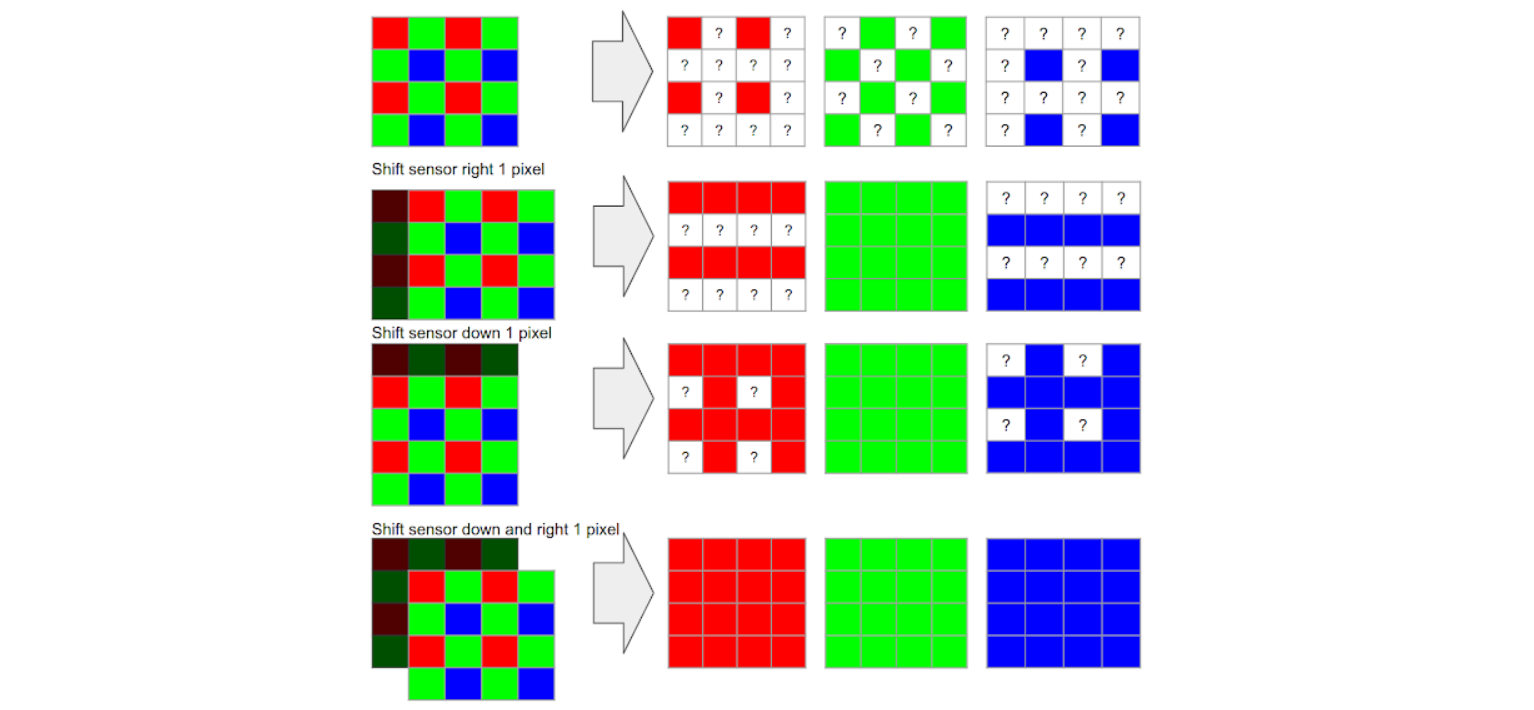
\includegraphics[width=\linewidth]{usecase.png}
      \caption{This algorithm is used to completely fill up the pixels.}
      \label{fig:Algo}
  \end{figure}
\end{frame}

\begin{frame}
  \LARGE{Any questions?}
\end{frame}

\end{document}

